\chapter{The UK Bombe}

\section{Motivating Example}

\section{Changes to Enigma}

Starting in 1940, the German's enhanced the security of their 
key distribution. As discussed in CITE the \emph{Grundstellung} rotor 
position was sent along with the daily key and an operator chose a \emph{Spruchschlusse} to 
encode twice at the start of a message. Later iterations of this protocol removed the \emph{Grundstellung}
from key sheets.
\\\\These new key sheets contained the following columns
columns \emph{Tag/Datum}, \emph{Walzenlage}, \emph{Ringstellung}, \emph{Steckerverbindungen}, and \emph{Kenngruppen} 
\\\\Notice the removal of the \emph{Grundstellung} as well as the addition of the \emph{Kenngruppen}. The \emph{Kenngruppen} were a set of 
four trigrams used to identify which setting was being used to encode a message, this is particularly useful if trying to decode a message using a prior day's key. 
The operator would choose a trigram from the the \emph{Kenngruppen}, append two letters to the front of the trigram,
and this five letter combination (known as the \emph{Buchstabenkenngruppe}) would preceed the message being sent. If a message
was sent in multiple segments, multiple \emph{Buchstabenkenngruppe} were used to start each segment.
\\\\When sending a message the operator was to use the following protocol
\begin{enumerate}[I.]
\item The time at which the message was sent is listed
\item The number of parts which the message contained is listed
\item Which message part is being sent is listed
\item The length of the message part (not including \emph{Buchstabenkenngruppe}) is listed
\item A \emph{Grundstellung} rotor position is chosen and listed 
\item A \emph{Spruchschlüssel} rotor position is chosen and encoded using the \emph{Grundstellung}, this is listed
\item The \emph{Buchstabenkenngruppe} is listed
\item The message part encoded using the daily key and the \emph{Spruchschlüssel} position is listed
\end{enumerate}
It is clear that with this protocol, the Polish Bomba could no longer deduce the necessary 
details to decrypt enigma messages. All of the permutation information contained in the original key distribution 
protocol was removed and a new method needed to be derived for infering information about the daily key.
\section{Loops}
The removal of the double encoded \emph{Spruchschlüssel} does not mean that permutation information cannot be stored elsewhere in the message. 
For the sake of argument, let us say we knew that our encrypted message had plaintext encoding

\begin{center}
\begin{tikzpicture}[node distance=1cm, every node/.style={draw, circle, minimum height=0.1cm, minimum width=0.1cm}]

    % Centering the diagram
    \node (a1) [] {D};
    \node (a2) [right=0.1cm of a1] {Y};
    \node (a3) [right=0.1cm of a2] {Y};
    \node (a4) [right=0.1cm of a3] {Y};
    \node (a5) [right=0.1cm of a4] {Y};
    \node (a6) [right=0.1cm of a5] {Y};
    \node (a7) [right=0.1cm of a6] {X };
    \node (a8) [right=0.1cm of a7] {Y};
    \node (a9) [right=0.1cm of a8] {Y};
    \node (a10) [right=0.1cm of a9] {Y};
    \node (a11) [right=0.1cm of a10] {X};
    
    % Nodes for ciphertext
    \node (x1) [below=1cm of a1] {A};
    \node (x2) [below=1cm of a2] {B};
    \node (x3) [below=1cm of a3] {R};
    \node (x4) [below=1cm of a4] {A};
    \node (x5) [below=1cm of a5] {C};
    \node (x6) [below=1cm of a6] {A};
    \node (x7) [below=1cm of a7] {D};
    \node (x8) [below=1cm of a8] {A};
    \node (x9) [below=1cm of a9] {B};
    \node (x10) [below=1cm of a10] {R};
    \node (x11) [below=1cm of a11] {A};
    
    % Arrows for mapping
    \draw[->] (a1) -- (x1) node[midway, left, draw=none, fill=none] {1};
    \draw[->] (a2) -- (x2) node[midway, left, draw=none, fill=none] {2};
    \draw[->] (a3) -- (x3) node[midway, left, draw=none, fill=none] {3};
    \draw[->] (a4) -- (x4) node[midway, left, draw=none, fill=none] {4};
    \draw[->] (a5) -- (x5) node[midway, left, draw=none, fill=none] {5};
    \draw[->] (a6) -- (x6) node[midway, left, draw=none, fill=none] {6};
    \draw[->] (a7) -- (x7) node[midway, left, draw=none, fill=none] {7};
    \draw[->] (a8) -- (x8) node[midway, left, draw=none, fill=none] {8};
    \draw[->] (a9) -- (x9) node[midway, left, draw=none, fill=none] {9};
    \draw[->] (a10) -- (x10) node[midway, left, draw=none, fill=none] {10};
    \draw[->] (a11) -- (x11) node[midway, left, draw=none, fill=none] {11};
    
    \end{tikzpicture}
\end{center}

Where the top row is the ciphertext and the bottom is the plaintext, further, the number in each mapping indicates how many steps away we are from the rotor 
positions when we began encoding the message.

\begin{center}
    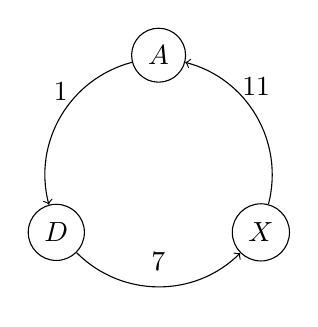
\begin{tikzpicture}[node distance=1cm, every node/.style={draw, circle, minimum height=0.1cm, minimum width=0.1cm}]
        \node (A) at (90:1.5) {$A$};
        \node (D) at (210:1.5) {$D$};
        \node (X) at (330:1.5) {$X$};
      
        \draw[->, bend right=45] (A) to node[midway, draw=none, above] {1} (D);
        \draw[->, bend right=45] (D) to node[midway, draw=none, above] {7} (X);
        \draw[->, bend right=45] (X) to node[midway, draw=none, above] {11} (A);
      \end{tikzpicture}
\end{center}

Recall
\begin{align*}
    E_1 &= P^{-1}\theta_1R_1^{-1}\theta_1^{-1}R_2^{-1}R_3^{-1}MR_3R_2\theta_1^{-1}R_1\theta_1P
    \\E_7 &= P^{-1}\theta_7R_1^{-1}\theta_7^{-1}R_2^{-1}R_3^{-1}MR_3R_2\theta_7^{-1}R_1\theta_7P
    \\E_{11} &= P^{-1}\theta_{11}R_1^{-1}\theta_{11}^{-1}R_2^{-1}R_3^{-1}MR_3R_2\theta_{11}^{-1}R_1\theta_{11}P
\end{align*}
Then it follows that our loop can be represented by 
\begin{align*}
    \sigma &= E_{11}\circ E_7 \circ E_{1}
\end{align*}
and we see that all the intermediate plugboard settings cancel out. Lets isolate the plugboard settings by letting 
$\overline{\sigma}$ represent $\sigma$ without the use of the plugboard for input and output, then 
\[
    \sigma = P^{-1}\overline{\sigma}P
\]
We have that
\begin{align*}
    \sigma(A) &= A
    \\\iff (P^{-1}\overline{\sigma}P)(A) &= A
    \\\iff \overline{\sigma}(P(A)) &= P(A)
\end{align*}

Suppose that our initial rotor position was correct, then certainly our $\overline{\sigma}$ is correct. We can make a hypothesis 
that $A$ is steckered to $K$ in the plugboard. Suppose we find that $\overline{\sigma}(K) \ne K$, then $\sigma(A)\ne A$ and our loop is broken, breaking our assumptions, thus $A$ must not be steckered to $K$.
But this will actually elimiate more hypotheses than just $A$ being steckered to $K$. We know that $\overline{\sigma}(K)$ is some letter which is not $K$. So we continue with a new hypothesis that $A$ is steckered to 
$\overline{\sigma}(K)$ and if we find $\overline{\sigma}(\overline{\sigma}(K)) \ne \overline{\sigma}(K)$, then we have further eliminated this possibility. 
Each new hypothesis suggests that $A$ is steckered to $\overline{\sigma}^{i}(K)$ which will be shown to be false if $\overline{\sigma}^{i+1}(K) \ne \overline{\sigma}^{i}(K)$. What if we find that 
$\overline{\sigma}^{i+1}(K) = \overline{\sigma}^i(K)$ at some point? This cannot happen since 
\begin{center}
        \begin{align*}
            &\overline{\sigma}^{i+1}(K) = \overline{\sigma}^i(K)
            \\\Rightarrow \text{ }&\overline{\sigma}^{-i}\circ\overline{\sigma}^{i+1}(K) = \overline\sigma^{-i}\circ\overline{\sigma}^i(K)
            \\\Rightarrow \text{ }&\overline{\sigma}(K) = K
        \end{align*}
\end{center}
which by supposition is false. Then we can continue in our hypotheses until we eventually reach a cycle where $\overline\sigma^i(K) = K$.
Then we gather a set of impossible steckerings, that is
\begin{align*}
    P(A) \notin \{\text{ }\overline{\sigma}^i(K)\text{ }\vert\text{ }i\in\mathbb{N}\}
\end{align*}
\\\\The notation we are using can be simplified significantly. The set $\{\text{ }\overline{\sigma}^i(K)\text{ }\vert\text{ }i\in\mathbb{N}\}$ is equivalent to the orbit of $K$ via the group action of the 
cyclic subgroup $\langle\overline{\sigma}\rangle$ which can be denoted $\langle\overline{\sigma}\rangle\cdot K$. 
\\\\We then have several cases 
\begin{enumerate}
    \item If $|\langle\overline{\sigma}\rangle\cdot K| = 26$, then $A$ cannot be steckered to anything which is clearly
    impossible, thus our rotor position must be incorrect. 
    \item If $|\langle\overline{\sigma}\rangle\cdot K| = 25$, then $A$ can only be steckered to the remaining letter \\$\{A,\dots,Z\} -
    \langle \overline{\sigma} \rangle\cdot K$
    \item If $|\langle\overline{\sigma}\rangle\cdot K| = 1$, in this case we must have intially had $\overline{\sigma}(K) = K$ so we have not
    eliminated any possibilities. 
\end{enumerate}

\section*{Motivating Example}

Suppose we knew the plaintext which had been enciphered into a particular enigma transmission.
Consider the following mapping,
\begin{center}
    \begin{tikzpicture}[node distance=1cm, every node/.style={draw, circle, minimum height=0.1cm, minimum width=0.1cm}]
    
        % Centering the diagram
        \node (a1) [] {D};
        \node (a2) [right=0.1cm of a1] {Y};
        \node (a3) [right=0.1cm of a2] {Y};
        \node (a4) [right=0.1cm of a3] {Y};
        \node (a5) [right=0.1cm of a4] {Y};
        \node (a6) [right=0.1cm of a5] {Y};
        \node (a7) [right=0.1cm of a6] {X };
        \node (a8) [right=0.1cm of a7] {Y};
        \node (a9) [right=0.1cm of a8] {Y};
        \node (a10) [right=0.1cm of a9] {Y};
        \node (a11) [right=0.1cm of a10] {X};
        
        % Nodes for ciphertext
        \node (x1) [below=1cm of a1] {A};
        \node (x2) [below=1cm of a2] {B};
        \node (x3) [below=1cm of a3] {R};
        \node (x4) [below=1cm of a4] {A};
        \node (x5) [below=1cm of a5] {C};
        \node (x6) [below=1cm of a6] {A};
        \node (x7) [below=1cm of a7] {D};
        \node (x8) [below=1cm of a8] {A};
        \node (x9) [below=1cm of a9] {B};
        \node (x10) [below=1cm of a10] {R};
        \node (x11) [below=1cm of a11] {A};
        
        % Arrows for mapping
        \draw[->] (a1) -- (x1) node[midway, left, draw=none, fill=none] {1};
        \draw[->] (a2) -- (x2) node[midway, left, draw=none, fill=none] {2};
        \draw[->] (a3) -- (x3) node[midway, left, draw=none, fill=none] {3};
        \draw[->] (a4) -- (x4) node[midway, left, draw=none, fill=none] {4};
        \draw[->] (a5) -- (x5) node[midway, left, draw=none, fill=none] {5};
        \draw[->] (a6) -- (x6) node[midway, left, draw=none, fill=none] {6};
        \draw[->] (a7) -- (x7) node[midway, left, draw=none, fill=none] {7};
        \draw[->] (a8) -- (x8) node[midway, left, draw=none, fill=none] {8};
        \draw[->] (a9) -- (x9) node[midway, left, draw=none, fill=none] {9};
        \draw[->] (a10) -- (x10) node[midway, left, draw=none, fill=none] {10};
        \draw[->] (a11) -- (x11) node[midway, left, draw=none, fill=none] {11};
        
        \end{tikzpicture}
    \end{center}
    where the top row indicates our enciphered message, the bottom row indicates the plaintext,
    and then indices on the arrows indicate how many steps forward our enigma machine has moved while enciphering this message.
    Our goal is to determine which enigma settings were used to encipher the message.  In order to achieve this, 
    we will examine which settings maintain the relationships between the enciphered and plaintext letters. 
    \\\\For example, any setting which maintains the above pairing must encipher $A$ to $D$ from the first position of the machine, then at 
    the seventh position, it must encipher $D$ to $X$, and at the eleventh position $X$ must be enciphered back to $A$. It follows that if we had 
    three enigma machines connected in series, with an offset of 1, 7, and 11, from our initial position, then inputting $A$ on the first machine would result in an ouput of $A$ on the
    third machine. We visualize this loop as follows 
    \begin{center}
        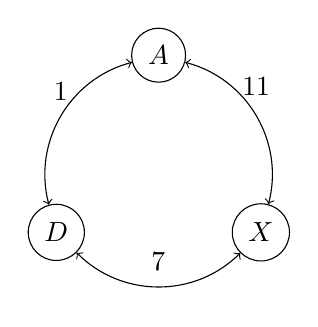
\begin{tikzpicture}[node distance=1cm, every node/.style={draw, circle, minimum height=0.1cm, minimum width=0.1cm}]
            \node (A) at (90:1.5) {$A$};
            \node (D) at (210:1.5) {$D$};
            \node (X) at (330:1.5) {$X$};
          
            \draw[<->, bend right=45] (A) to node[midway, draw=none, above] {1} (D);
            \draw[<->, bend right=45] (D) to node[midway, draw=none, above] {7} (X);
            \draw[<->, bend right=45] (X) to node[midway, draw=none, above] {11} (A);
          \end{tikzpicture}
    \end{center}
    To express this mathematically we denote the permutation represented by the enigma at 
    position $i$ as $\sigma_i$. Since these each use the same plugboard we will also note the 
    enigma at position $i$ not using the plugboard as $\overline{\sigma_i}$, that is $\sigma_i = P\overline{\sigma_i}P$.
    Then our loop is expressed by the fact that $\sigma_{11}\circ\sigma_7\circ\sigma_1$ has a fixed point at $A$. 
    We also note that the intermediate plugboard settings cancel out, that is 
    \begin{center}
        \begin{align*}
            \sigma_{1}\circ\sigma_7\circ\sigma_{11} &= P\overline{\sigma_{1}}P\circ P\overline{\sigma_7}P\circ P\overline{\sigma_{11}}P
            \\&= P\circ \overline{\sigma_{1}}\circ\overline{\sigma_7}\circ\overline{\sigma_{11}}\circ P
        \end{align*}
    \end{center}
    We will condense this notation by defining
    \begin{center}
        $\sigma \coloneq \sigma_{1}\circ\sigma_7\circ\sigma_{11}$
    \end{center}
    and 
    \begin{center}
        $\overline{\sigma} \coloneq \overline{\sigma_{1}}\circ\overline{\sigma_7}\circ\overline{\sigma_{11}}$
    \end{center}
    And thus we have shown $\sigma = P\overline{\sigma}P$.
    \\\\Let us hypothesize that $A$ is steckered in the plugboard $\alpha$ -- that is, $P(A) = \alpha$. It then follows that 
    \begin{center}
        \begin{align*}
            \overline{\sigma}^i(\alpha) &= P\circ\sigma^i\circ P(\alpha)
            \\&= P\circ\sigma^i(A)
            \\&= P(A)
        \end{align*}
    \end{center} 
    and so we derive 
    \begin{center}
        $P(A) = \alpha \Rightarrow P(A) = \overline{\sigma^i}(\alpha)\text{ }\forall\text{ }i\in\mathbb{N}$
    \end{center}
    Then we have that $A$ must be steckered to all values in the set $\{\overline{\sigma}^i(\alpha)\text{ }\vert\text{ }i\in\mathbb{N}\}$. 
    We note that this set is that orbit of the element $\alpha$ under the group action of the subgroup $\langle\overline{\sigma}\rangle$ -- that is, 
    $\langle\overline{\sigma}\rangle\cdot\alpha$. 
    \\\\By construction of the enigma machine, $A$ cannot be steckered to more than one value at a time, so if $|\langle\overline{\sigma}\rangle\cdot\alpha| > 1$ our initial
    hypotheses that $P(A) = \alpha$ must have been incorrect. Further, the above arugment also illustrates that $A$ cannot be steckered to any element in the orbit of $\alpha$ since 
    we would similarly find that the orbit of that element was not a singleton. Then we now have 
    \begin{center}
        $|\langle\overline{\sigma}\rangle\cdot\alpha| > 1 \Rightarrow P(A) \notin \langle\overline{\sigma}\rangle\cdot\alpha$
    \end{center} 
    thus eliminating several elements that $A$ could be steckered to. 
    \\\\In fact, if $|\langle\overline{\sigma}\rangle\cdot\alpha| = 26$
    then $A$ cannot be steckered to \emph{any} element. Of course, by construction, $A$ must be steckered to \emph{some} element, so it must be the case
    that this rotor position is impossible since no plugboard setting could produce the loop relationship in our ciphertext-plaintext pairing. 
    \\\\This is the 
    key idea in the construction of the Bombe. At a high level, we encode the structure of the ciphertext-plaintext pairings, we input a hypothesis that a particular 
    letter (e.g $A$) is steckered to another (e.g. $\alpha$), and we electrically produce the elements that must also be steckered to our test letter 
    (e.g. $\langle\overline{\sigma}\rangle\cdot\alpha$) if our hypothesis were to be true. If we find that this production generates a set of all letters and thus disqualifies this rotor position from producing
    the plaintext we observed, then we can continue on to the next rotor position until we have no contradictory results from our hypothesis.
    \\\\Before describing the function of the machine more concretely, we will first examine how we as humans can examine such permutations and deduce hypotheses quickly. 
    
    \section{The Bombe}

    In the section, we outline the construction of a rudementary Bombe. Our goal is to construct a machine using the above insight to quickly elimate a rotor position based on contradictory hypotheses. For clarity sake, we will 
    imagine that our Engima machine operates on an alphabet of only four letters $\{A, B, C, D\}$.  
    We must shift from the above mathematical construction to an electrical one. We first abstract the idea of the Engima machine and do away with the input output system of keys and lamp lights.
    Rather, we imagine the Enigma machine as black-box that takes in 4 cables encoding, via current, each of the 4 letters, and outputs currents on the corresponding letter after applying the Enigma permutation.
    Imagine the following set of wires encoding a possible Enigma permutation we will denoted $\overline\sigma_\alpha$ (the bar indicates we are not yet considering the plugboard).
    
    \tikzset{big box/.style={draw, minimum width=5cm, minimum height=4cm},
    small box/.style={draw, minimum width=1cm, minimum height=1cm}}

    \begin{center}
        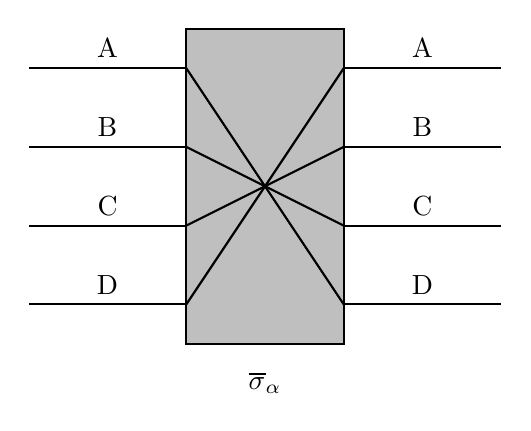
\begin{tikzpicture}[thick]
            % Draw the box
            \draw[fill=lightgray] (2,-1.5) rectangle (4,2.5) node[midway] {};
            
            \node at (3, -2) {$\overline\sigma_\alpha$};

            % Draw the wires entering the box
            \draw[-] (0, 2) -- (2, 2) node[midway, above] {A};
            \draw[-] (0, 1) -- (2, 1) node[midway, above] {B};
            \draw[-] (0, 0) -- (2, 0) node[midway, above] {C};
            \draw[-] (0,-1) -- (2,-1) node[midway, above] {D};

            % Draw the wires exiting the box with crossed mappings
            \draw[-] (4, 2) -- (6,2) node[midway, above] {A};
            \draw[-] (4, 1) -- (6, 1) node[midway, above] {B};
            \draw[-] (4, 0) -- (6, 0) node[midway, above] {C};
            \draw[-] (4,-1) -- (6, -1) node[midway, above] {D};

            % Draw the lines inside the box to represent the mapping
            \draw[-] (2, 2) -- (4,-1);
            \draw[-] (2, 1) -- (4, 0);
            \draw[-] (2, 0) -- (4, 1);
            \draw[-] (2,-1) -- (4, 2);

        \end{tikzpicture} 
    \end{center}
    A couple quick notes about this abstraction. First as these lines are simply wires, current can flow in either direction, left-to-right, or right-to-left. 
    Second, we can apply current to multiple wires concurrently, for example, applying current at $A$ and $C$ will cause $D$ and $B$ to be live on the other side of the machine.
    \\\\As described in our motivating example, we may want to connect Engima permutations in series to capture an underlying relationship between a ciphertext-plaintext pairing. 
    Suppose analysis found that we have three Enigma permutations represented by $\overline\sigma_\alpha, \overline\sigma_\beta$, and $\overline\sigma_\gamma$ which form a loop having a fixed point at $A$. 
    \begin{center}
    \begin{tikzpicture}[thick, scale=0.75, every node/.style={scale=0.7}]
        % Define the positions for the three diagrams in a circle
        \foreach \x/\y/\label/\mapping in {0/4/{$\alpha$}/ {(4,-1), (4,0), (4,1), (4,2)},
        -4/-2.5/{$\beta$}/ {(4,-1), (4,0), (4,1), (4,2)},
        4/-2.5/{$\gamma$}/ {(4,-1), (4,0), (4,1), (4,2)}} {
            \begin{scope}[shift={(\x,\y)}]
                % Draw the box
                \draw[fill=lightgray] (2,-1.5) rectangle (4,2.5) node[midway] {};
            
                % Label the box with sigma below
                \node at (3, -2) {$\overline\sigma_{\text{A}}$};
    
                % Draw the wires entering the box
                \draw[-] (0, 2) -- (2, 2) node[midway, above] {A};
                \draw[-] (0, 1) -- (2, 1) node[midway, above] {B};
                \draw[-] (0, 0) -- (2, 0) node[midway, above] {C};
                \draw[-] (0,-1) -- (2,-1) node[midway, above] {D};
    
                % Draw the wires exiting the box with crossed mappings
                \draw[-] (4, 2) -- (6,2) node[midway, above] {A};
                \draw[-] (4, 1) -- (6, 1) node[midway, above] {B};
                \draw[-] (4, 0) -- (6, 0) node[midway, above] {C};
                \draw[-] (4,-1) -- (6, -1) node[midway, above] {D};
    
                \foreach \endX/\endY in \mapping {
                    % Extract start and end coordinates from the mapping list
                    \pgfmathsetmacro{\startX}{2}
                    \pgfmathsetmacro{\startY}{2 - \i + 1}
                    \draw[-] (\startX, \startY) -- (\endX, \endY);
                }
                % Draw the lines inside the box to represent the mapping
            \end{scope}
            \draw[-] (0, 6) to[out=180, in=180] (-4, -0.5); % Connect A
            \draw[-] (0, 5) to[out=180, in=180] (-4, -1.5); % Connect B
            \draw[-] (0, 4) to[out=180, in=180] (-4,-2.5); % Connect C
            \draw[-] (0, 3) to[out=180, in=180] (-4,-3.5); % Connect D

            \draw[-] (0, -0.5) -- (6, -0.5); % Connect A
            \draw[-] (0, -1.5) -- (6, -1.5); % Connect A
            \draw[-] (0, -2.5) -- (6, -2.5); % Connect A
            \draw[-] (0, -3.5) -- (6, -3.5); % Connect A

            \draw[-] (6, 6) to[out=360, in=360] (10, -0.5); % Connect A
            \draw[-] (6, 5) to[out=360, in=360] (10, -1.5); % Connect B
            \draw[-] (6, 4) to[out=360, in=360] (10,-2.5); % Connect C
            \draw[-] (6, 3) to[out=360, in=360] (10,-3.5); % Connect D
        }
    \end{tikzpicture}
\end{center}
    \section{Cycles}
    Another way of viewing the orbit of the element $\alpha$ under the action by $\langle\overline\sigma\rangle$ in our motivating example, is to consider the cycle in $\overline\sigma$ containing $\alpha$.
    Suppose our alphabet had six letters $\{\alpha, \beta, \gamma, \delta, \epsilon, \zeta\}$. We may find that in our cycle notation we can write $\overline\sigma$ as 
    \begin{center}
        $(\alpha\beta\gamma)(\delta\epsilon)(\zeta)$
    \end{center}
    From this, we can determine that had our hypotheses been that $P(A) = \alpha$ we would find that $P(A) = \beta$ and $P(A) = \gamma$. 
    Similarly, had we hypothesized that $P(A) = \delta$ we would have found that $P(A) = \epsilon$. This is to say, if we hypothesize that $P(A)$ is mapped to a particular
    element, then it must also be mapped to all elements in the cycle containing that element. 

  